\begin{flushleft}
    \section{Analysis} 
        \subsection{Statement Of Problem}
        \large
        \bk
        Maps, as you would think of them today, have been around since 6\textsuperscript{th} century BC and since then have been in constant use by people in their day to day lives. 
        The more modern version of maps, for example Google maps or Bing maps have only been around since the late 1990's. The problem that I am going to be solving is map path finding.
        Currently not all roads and paths are logged and entered into a searchable format. The only way some people have to navigate terrain is through the use of old style paper maps.
        The problem with paper maps is that they are not easily, at a glance, used to find a path from point to point. As well as this sometimes are not easy to comprehend just by looking 
        at them with various terrain features. \\
        
        \bk
        \begin{figure}[h]
            \centering
            \subfloat[\centering Map without labels on roads]{{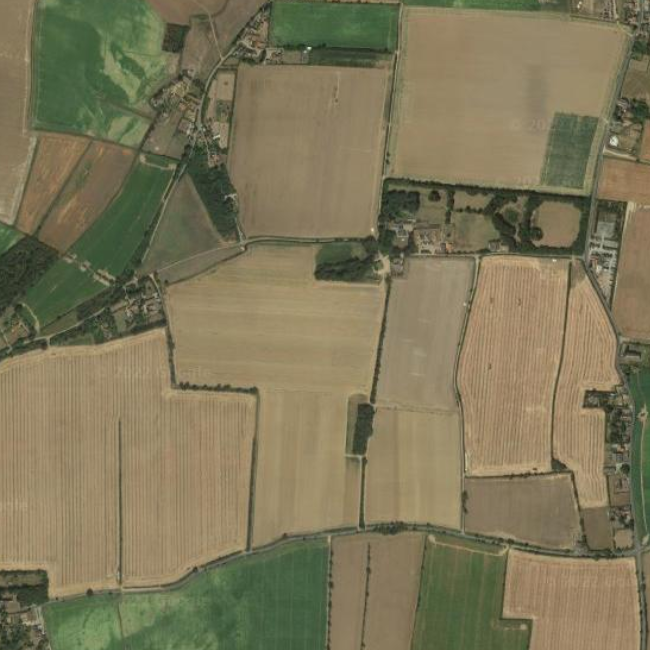
\includegraphics[width=6cm]{images/unlabeledMap.png}}}
            \qquad
            \subfloat[\centering Map with labels on roads]{{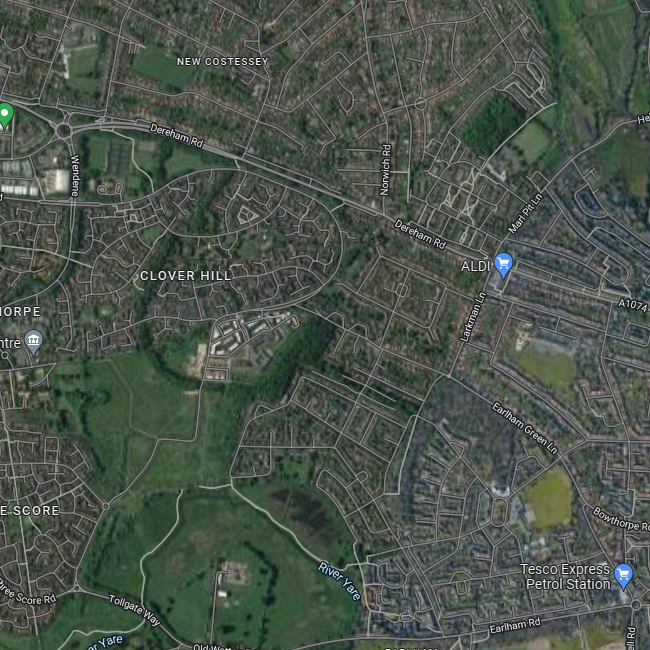
\includegraphics[width=6cm]{images/labeledMap.png}}}
            \caption*{Examples of maps with and without labels taken from Google Maps\textsuperscript{\textcopyright}}
        \end{figure}
        \bk

        This can cause issues for people who live out in areas which have not been mapped. This is because they cannot create easy to follow routes with the click of a button. Therefor, 
        causing people who live in rural areas to waste time getting used to the routes they have to take to go anywhere. Overall, the problem I am going to be creating a solution for is 
        how people are unable to easily go from point to point at the click of a button and be easily able to, at a glance, interpret the map without prior experience. \\

        \subsection{Background}
        \bk
        When people usually want to go about planning a journey they will use a service, for example Google Maps to get from one location to another. This usually takes the form of clicking 
        a location and then selecting an origin. This isn't always possible however, this can be for a multitude of reasons it seems however I will briefly go over some below:\\
        
        \begin{enumerate}
            \item \textbf{Either the destination or origin location(s) are not in the service's database.}
            \item \textbf{The destination and origin have no clear defined path between them.}
            \item \textbf{Either the destination or origin are off any predefined track.}
            \item \textbf{The travel method the user has selected is not able to traverse the terrain between the origin and destination.}
        \end{enumerate}

        \bk
        Some of these I believe are out of the scope of this project however once the interview has been conducted with the end user I will have a better idea of the needs that my program needs to for-fill.\\

        \bk
        Finally, 

        \bk
        
        \subsection{End User}
            \subsubsection{First Interview}
            \large
            In order to get a better feel for the objectives and functions that my program should complete I interviewed with an end user, Mrs Mandy T. I believed that she was an appropriate candidate for this
            project due to the fact that she has to drive into work every morning. Along her route she has to deal with Google Maps which do not cover all of the roads in her area. Therefor in the following questions
            I asked her some questions gauge her priorities when it comes to web mapping.
            \bk
            \begin{enumerate}
                \item {\bf{When using web maps (e.g. Google Maps\textsuperscript{\tiny\textcopyright}) what are the key features you look for?}} \\
                \bk
                "A scale! WHY is it lost so often when Google Maps is embedded?! 
                Then it depends what type of map I'm looking at... if it's a road map then....roads! Size/type of road is important and things like one-way restrictions. 
                If it's for e.g. walking...footpaths/bridleways and parking are important. 
                "
                \item {\bf{Have you ever experienced a faulty or mislabeled part of an web map or has said map ever been inaccurate?}} \\
                \bk
                "Yes"
                \item {\bf{Do you often use web maps in your day to day life, if so how?}} \\
                \bk
                "Yes, \textbf{NEEDS TO BE ADDED TO}"
                \item {\bf{In your opinion do you feel that web maps are vital to every day life if so why or why not? }} \\
                \bk
                "No.  I passed my driving test before we had sat-nav or internet, so clearly they're not vital - we survived without them! \\ 
                They are quite helpful though as we used to have to buy a new road map every year, whereas web maps can be updated as things change, instead of only annually!"
                \item {\bf{What makes a good user interface for a web map?}} \\
                \bk 
                "Clarity and simplicity.  Nothing needlessly complicated."
                \item {\bf{How do you use web maps (e.g. long journeys, short journeys, school runs)?}} \\
                \bk
                "Route functionality on long or unfamiliar journeys. 
                Using them a lot at the moment as am planning a holiday overseas.  The maps are useful to see whether accommodation and restaurants will be walking distance, 
                and what options there are in each location etc."
                \item {\bf{Do you feel a tutorial would be beneficial to aid in the use of the map or should the focus more be spent on intuitive ease of use?}} \\
                \bk
                "If they're easy to use, a tutorial would be surplus to requirements, so ease of use is more important. "
                \item {\bf{Would it be beneficial to store old routes?}} \\
                \bk
                "Not really (is this a routing question?). I don't know what purpose that would give, unless I was being accused of something and needed to use the route as evidence of 
                being in a certain location! It could be use full in the context of frequently traveled routes however if this was the case I would know the route by heart anyway."
                \item {\bf{What forms of transport should the map include?}} \\
                \bk
                "(I think this is a routing question not a map question)
                Walking, bike/horse, car, bus, plane, ferry. 
                If just a map question, then the map should include footpaths, bridle paths, roads, ferry routes"
                \item {\bf{If there was one feature you could have implemented in an existing solution what would it be?}} \\
                \bk
                "To be able to post a question about a specific area and have a person who is local to that area answer it."
            \end{enumerate}
            
            \subsubsection{Evaluation of First Interview}
            Overall I feel that this interview gave me valuable insight into the requirements of my end user. As well as this my end user made it clear to me that there are two overriding 
            parts of this solution. The map recognition aspect of it and the path finding aspect. Going deeper into the path finding part of this project I will need to do research on the 
            different methods that will be used to achieve this and some of the possible data structures I could use. \\
        \bk

        \subsection{Initial Research} 
            \subsubsection{Existing Solutions}
            Below each overview passage I have included an image of each map for comparison of their GUI's. These will be used as inspiration as to how my final solution will look as well 
            as serving as examples of how the GUI can sometimes become overly complicated. This is especially the case with Bing Maps as when you initially access it you are flooded with 
            popups and extra options. \\
            \paragraph{Google Maps} \mbox{} \\
            \bk
            
            As aforementioned this is one of the most used forms of interactive web mapping in use at the moment. It has been in use since 8\textsuperscript{th} February 2005. As it exists
            now it is an interactive world map with routing features built in. It provides detailed information about geographical places and regions around the world. Unlike some of its
            competitors it also offers aerial and satellite images of places around the world aiding in navigation of terrain. \\
            
            \bk
            
            As well as its map viewing capabilities it also offers partial route planning and live route tracking for cars, bikes, walkers and public transport. It provides instantaneous and
            real time feedback while you are moving however the one big caveat to this is the fact that it will require an internet connection to run, something that is not always available. \\
            \bk
            
            \begin{figure}[H]
                \centering
                \subfloat[\centering Example of Google Maps' GUI]{{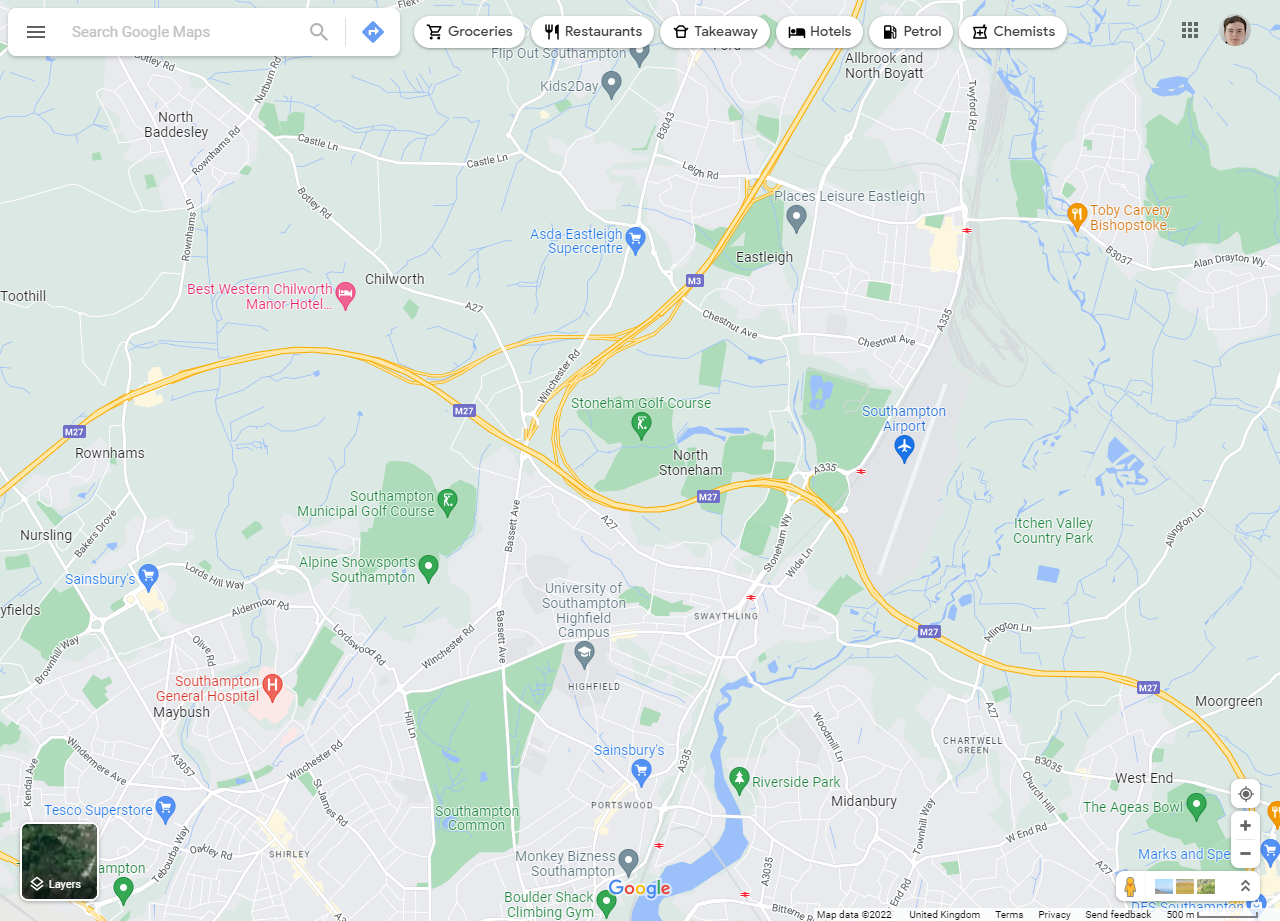
\includegraphics[width=10cm]{images/googleMapExample.png}}}
                \caption*{Sourced from Google Maps\textsuperscript{\tiny\textcopyright}}
            \end{figure}

            \bk 
            
            \paragraph{Bing Maps} \mbox{} \\
            This is another form of interactive web mapping. This is a more plain version of Google Maps at first glace. This is due to the fact that it does not have as many features as Google Maps.
            This does have its advantages due to the UI seeming less cluttered and more accessible. Similar to the Google Maps it also offers route planning and map traversal as well as live traffic updating.
            Bing maps unlike Google Maps boasts a more open API and easier programmatic interface for developers to be able to interface with their program. \\
 
            \bk
 
            Bing maps also still includes the feature which allows users to create their own maps based on their own data. Unlike google which did have this feature until they discontinued it.
            I believe that this could be something that would be beneficial to my program, allowing people to take a photo of their own map and have my solution compute it into a routable map. \\
 
            \bk
 
            \begin{figure}[H]
                \centering
                \subfloat[\centering Example of Bing Maps' GUI]{{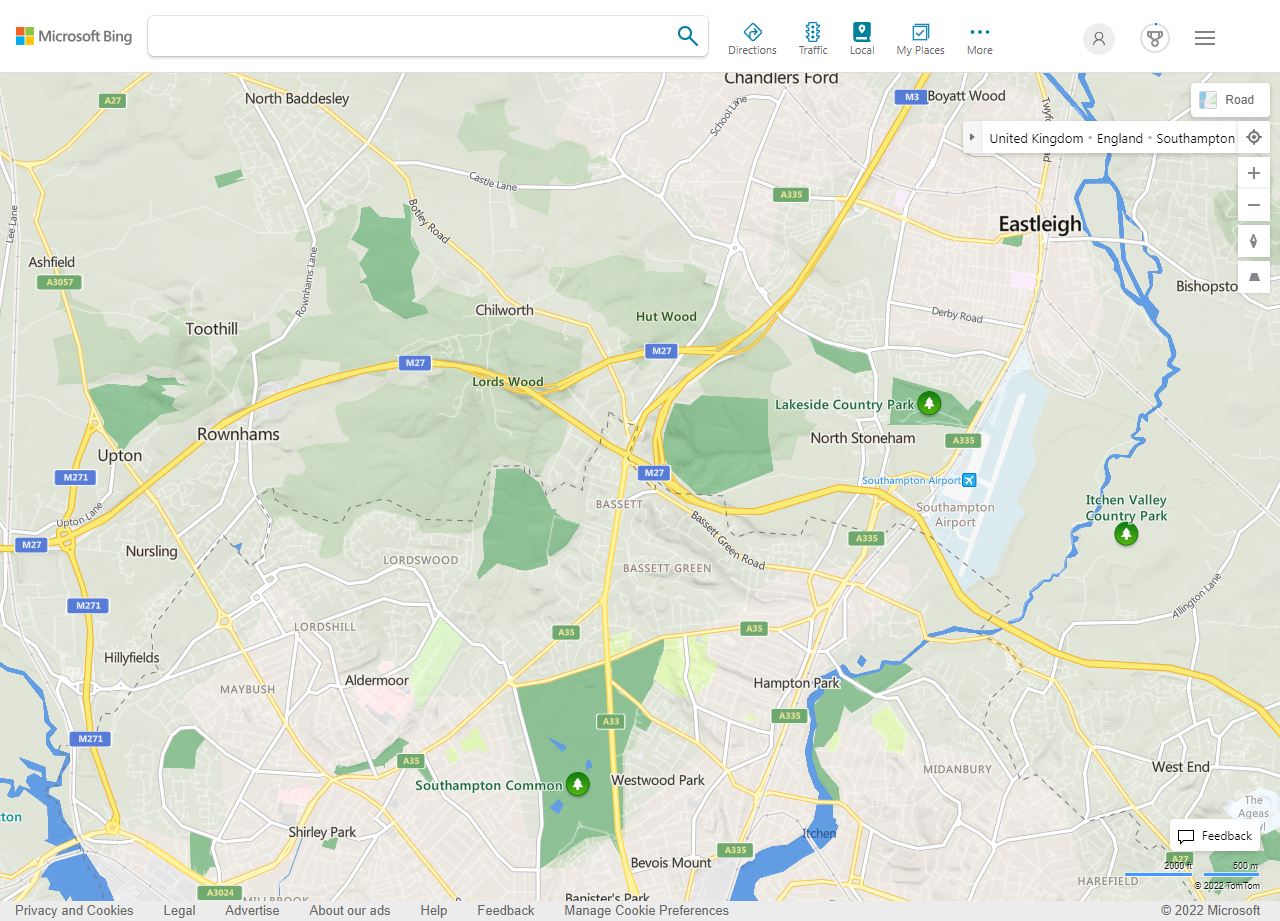
\includegraphics[width=10cm]{images/bingMapExample.png}}}
                \caption*{Sourced from Bing Maps\textsuperscript{\tiny\textcopyright}}
            \end{figure}

            \bk

            \paragraph{OS Maps} \mbox{} \\
            This is a different take in web mapping compared to Bing and Google Maps. With Ordnance Survey their focus was on the accuracy of their maps hence they do not have as an extensive routing system.
            If you wanted to go from point to point on an OS map you would have to plot it by hand. However if you wanted to go on an exercise trail on the other hand they are very well suited
            for this and as such have an extensive list of pre-planned routes. \\
            \bk
            Similar to Google Maps, and in a limited capacity, Bing maps; OS Maps allow you to view their maps in different forms such as 3D and topographic however in order to access these you will
            have to access their premium plan therefor for the average user this is not a viable option and a hindrance. It is good to note however that the other variations on the map of the UK,
            and this holds true for all of the aforementioned maps, that the satellite view and other views are not necessary and could in fact be a hindrance. \\
            
            \bk
            
            \begin{figure}[H]
                \centering
                \subfloat[\centering Example of Ordnance Survay's Map GUI]{{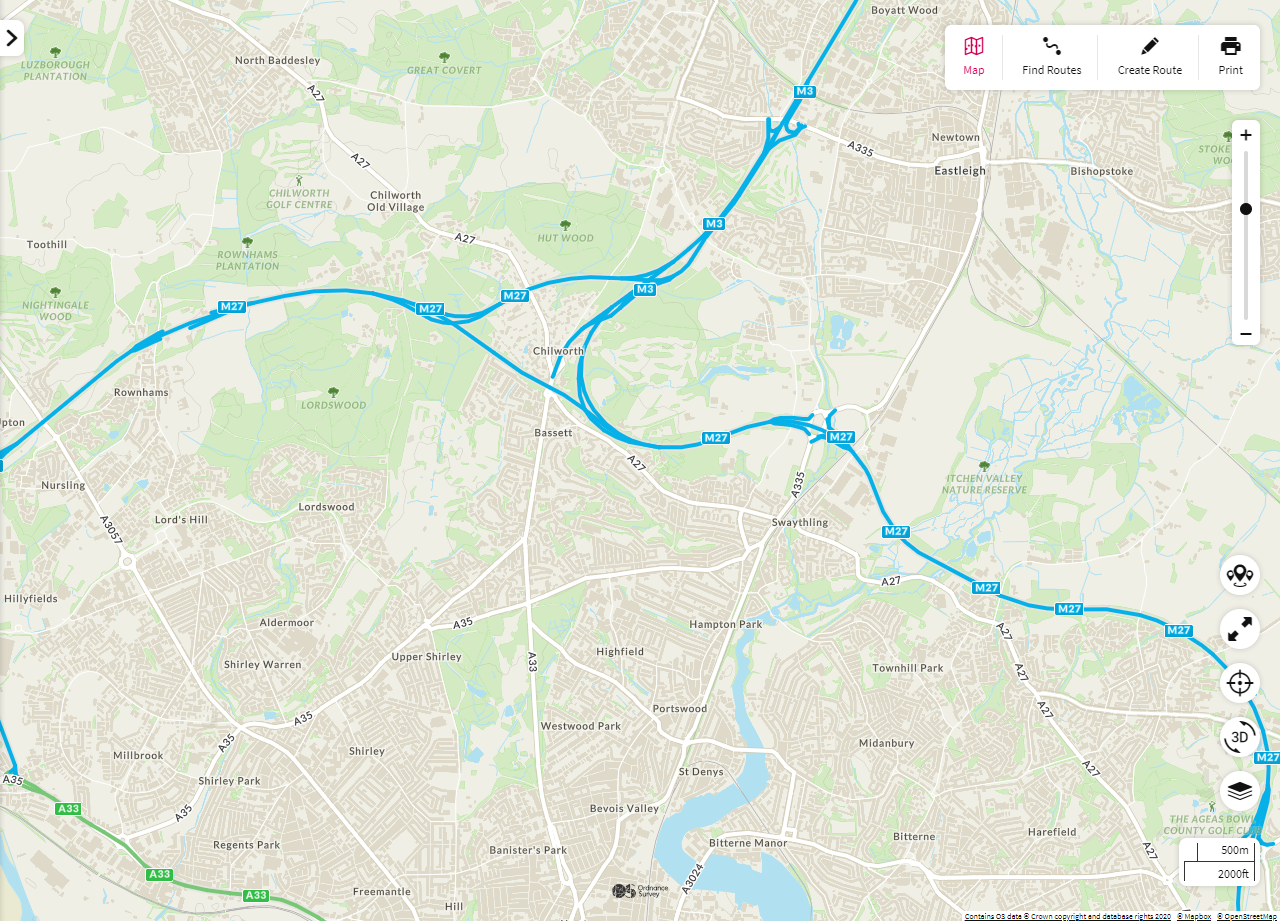
\includegraphics[width=10cm]{images/osMapExample.png}}}
                \caption*{Sourced from Bing Maps\textsuperscript{\tiny\textcopyright}}
            \end{figure}

            \bk
            
            \paragraph{Existing Solutions Conclusion} \mbox{} \\
            In conclusion, I have found that the existing solutions that are available are all very well designed and well implemented. I have found that they are easy to use and rather intuitive
            however, for the average user who just needs to get from A to B in the most economic way possible they are overly complicated. As well as this I have found that with the exception of OS maps
            both of the other solutions require an internet connection to get the best use out of their maps, this is something which I believe I should avoid. This will mean that all calculations will 
            have to occur self contained within the program, not allowing the use of external API's. \\
            \bk

            \subsubsection{Possible Algorithmic Solutions}
            There are\dots
            \bk

            \subsubsection{Key Components Required}
            \paragraph{Graphical User Interface} \mbox{} \\
            \bk
            \paragraph{Image Manipulation} \mbox{} \\
            \bk
            \paragraph{Graph Creation / Theory} \mbox{} \\
            \bk
            \paragraph{Various Traversal Algorithms} \mbox{} \\
            \bk


        \subsection{Further Research}
            \subsubsection{Dive into Specific Algorithms}
            After doing some research it seems that there needs to be a set of definitions before I go any further to avoid confusion. This is because during my time on Wikipedia there are sections
            where several terms are used interchangeable where I feel they are not the same. Each of these definitions are as defined by me and are not necessarily the official definitions since they 
            do not explicitly exist. They are as follows: \\ \bk
            \begin{enumerate}
                \item Graph Traversal: The act of routing or searching through a graph from one node to another, either using an algorithm or by another means.
                \item Graph Routing: Graph traversal in a \emph{weighted undirected} graph.
                \item Graph Searching: Graph traversal in a \emph{unweighted undirected} graph.
                \item Graph MST: The minimum spanning tree of a graph which must be weighted.
            \end{enumerate}

            \bk

            The difference is slight however the key takeaway from this is that when I am referring to a Routing algorithm I am referring to one which works on a weighted graph. And vice versa if I am
            talking about a searching algorithm this is referring to graph traversal on an unweighted graph.

            \bk

            \paragraph{Black and White Filter}
            \mbox{} \\
            
            \bk
            $
                \mathlarger {
                    \beta = 0.299 * \alpha_{b} + 0.587 * \alpha_{g} + 0.114 * \alpha_{b}
                }
            $
            \bk
            \\
            \bk
            $
                \beta = \begin{cases}
                    255 & \beta > 255 \\
                    0 & \beta < 0 \\
                    \beta & \beta \in [0, 255]
                \end{cases}
            $
            \bk

            \bk
            \paragraph{Gaussian Filter}
            \mbox{} \\
            
            \bk
            $
                H_{ij} = \frac{1}{2\pi\sigma^{2}} \exp \bigg(-\frac{(i - (k + 1))^{2} + (j - (k + 1))^{2}}{2\sigma^{2}}\bigg);1\leq i, j \leq(2k+1)
            $
            \bk
            \\
            \bk

            \subsubsection{Second Interview}
            \large
            Now that I have done some more research into the various ways there are to complete this task I have formed some more questions to ask my end user to get a solid and
            defined list of objectives for the program. AI will couple this with my research to form a complete plan to form said objectives. As well as this however the second interview
            will allow me to correct any inaccurate questions that where asked in the initial interview. This is because after I received my initial responses I realised that I
            needed to be more clear with what I was asking and the information that I wanted back. \\
            \bk
            
            \begin{enumerate}
                \item {\bf{Bobbert?}} \\
                \bk
                bobbert.
                \item {\bf{Bobbert?}} \\
                \bk
                bobbert.
                \item {\bf{Bobbert?}} \\
                \bk
                bobbert.
                \item {\bf{Bobbert?}} \\
                \bk
                bobbert.
                \item {\bf{Bobbert?}} \\
                \bk
                bobbert.
                \item {\bf{Bobbert?}} \\
                \bk
                bobbert.
                \item {\bf{Bobbert?}} \\
                \bk
                bobbert.
            \end{enumerate}

            \subsubsection{Evaluation of Second Interview}
            After conducting this second interview I feel I now have a firm understanding of what I need to achieve with this program. I will also take this opportunity to create a prototype of the 
            the different parts of the program to gauge the difficulty of the program and any problems I may encounter before moving onto the final solution. \\ \bk
            Apart from that however I feel the interview went\dots

        \subsection{Objectives}
        \large
        
        % Tips for objectives
        
        % 1. Use numbered objectives to allow them to be refer ed back to
        % 2. Don't mention programming techniques
        % 3. Objectives for the program not the programmer
        
        After conducting the initial and second interviews and reflecting upon the results of my research I have formed a list of objectives that the program must meet to be considered 
        complete. As well as the base objectives I have also, with help from my end user, come up with extensions which will increase the effectiveness of my solution overall. \\
        \bk
        
        \renewcommand{\labelenumii}{\arabic{enumi}.\arabic{enumii}}
        \renewcommand{\labelenumiii}{\arabic{enumi}.\arabic{enumii}.\arabic{enumiii}}
        \renewcommand{\labelenumiv}{\arabic{enumi}.\arabic{enumii}.\arabic{enumiii}.\arabic{enumiv}}
        
        \begin{enumerate}
            \item The Program must have way to input a Map
            \begin{enumerate}
                \item The Program should be able to parse a map from a file, including
                \begin{enumerate}
                    \item A photograph of an map
                    \item A screenshot of an existing map
                    \item A hand drawing of suitable quality
                \end{enumerate}
                \item When the user inputs a map, the program will ask them
                \begin{enumerate}
                    \item What type of map they are inputting
                    \item How they would like the result of the map
                    \item How harsh they would like the edge detection to be
                    \item The resolution of which to parse the map too
                    \item Whether they would like to path find through the map or form a Graph MST
                    \item \emph{These are some examples of prompts}
                \end{enumerate}
                \item The inputted map should be converted into a graph
                \item The map (in graph form) should be able to be traversed
                \item If any error occurs during the map input process an appropriate error should be displayed and the program should continue to run
            \end{enumerate}
            
            \item The Program must allow Map Traversal
            \begin{enumerate}
                \item There should be Multiple Traversal Algorithms Available to be chosen from.
                    \begin{enumerate}
                        % https://en.wikipedia.org/wiki/Category:Graph_algorithms
                        \item The Program should implement Routing Algorithms 
                        \begin{enumerate}
                            \item This includes Dijkstra's algorithm
                            \item This includes A*
                            \item This includes
                        \end{enumerate}
                        % https://en.wikipedia.org/wiki/Category:Search_algorithms
                        \item The Program should Implement Searching Algorithms
                        \begin{enumerate}
                            \item This includes BFS (Breadth-first search)
                            \item This includes DFS (Deapth-first search)
                            \item This includes Greedy Best-First Search
                        \end{enumerate}
                        \item The program should implement a Minimum spanning tree
                        \begin{enumerate}
                            \item It should implement Primm's algorithm
                            \item It should implement Kruskal's algorithm
                        \end{enumerate}
                    \end{enumerate}
                \item Depending on the option that the user chooses they can either
                \begin{enumerate}
                    \item Decide a specific algorithm to use
                    \item Have the program compute all and use the most efficient one
                    \item Have the program compute all and let the user select one
                \end{enumerate}
            \end{enumerate}
            
            \item The Program must have a Clear and Simplistic GUI
            \begin{enumerate}
                \item At a glance the user should be able to accertain which step they are at.
            \end{enumerate}

            \item The Program must have image processing capabilities
            \begin{enumerate}
                \item The program should be able to perform edge Detection
            \end{enumerate}
            \bk          
        \end{enumerate}  
        
        \vspace{1cm}
        \centerline{\large\textbf{Extension Objectives}}
        \vspace{1cm}

        \begin{enumerate}[resume]
            \item The program should be able to be output
        \end{enumerate}

        \bk

        \subsection{Modeling}
        \bk

\end{flushleft}